\documentclass[fleqn,t]{beamer}
\usetheme{boxes}

\title{Fast Decision Procedures Based on Congruence Closure}
\subtitle{Greg Nelson and Derek C. Oppen}
\author{Sven Keidel}
\date{\today}

\usepackage[utf8]{inputenc}

\usepackage{fancyvrb}
\usepackage[cache]{minted}
\newmintedfile{haskell}{ fontsize=\footnotesize }

\usepackage{tikz}
\usetikzlibrary{arrows,calc,positioning,decorations.pathmorphing}
\tikzstyle{vertex}=[circle,draw,minimum size=0.7cm]
\tikzstyle{edge}=[->, >=latex,draw]
\tikzstyle{equal}=[-, >=latex,dashed,draw]
\tikzset{
  invisible/.style={opacity=0},
  visible on/.style={alt={#1{}{invisible}}},
  alt/.code args={<#1>#2#3}{
    \alt<#1>{\pgfkeysalso{#2}}{\pgfkeysalso{#3}}
  },
  only/.code args={<#1>#2}{
    \only<#1>{\pgfkeysalso{#2}}
  },
  beameralert/.style={only=<#1>{ultra thick,red},visible on=<#1->}
}

\newcommand{\car}[1]{\ensuremath\mathit{car}(#1)}
\newcommand{\cdr}[1]{\ensuremath\mathit{cdr}(#1)}
\newcommand{\cons}[1]{\ensuremath\mathit{cons}(#1)}
\newcommand{\atom}[1]{\ensuremath\mathit{atom}(#1)}
\newcommand{\nil}[0]{\ensuremath\mathit{nil}}

\begin{document}

\maketitle

\section{Introduction}

\begin{frame}
  \frametitle{Objective and Motivation}

  \begin{itemize}
    \item Decision procedure for the quantifier-free theory of equality with
      uninterpreted function symbols.
      \begin{itemize}
        \item $f(a,b) = a \rightarrow f(f(a,b),b) = a$
        \item $0 = 1$
      \end{itemize}

    \item Determines the satisfiability of a conjunction of
      literals of length $n$ in $O(n \log n)$.

    \item Can be extended to advanced theories like the theory of
      list-structures.
  \end{itemize}

\end{frame}


\subsection{Definitions}

\begin{frame}
  \frametitle{Term Graph}

  \begin{Definition}[Term Graph]
    \begin{itemize}
      \item Let $G = (V,E)$ be a directed graph.
      \item Let $\lambda(v)$ be the label of a vertex $v$.
      \item Let $\sigma(v)$ be the out degree of a vertex $v$.
      \item Outgoing edges are ordered. Let $v[i]$ denote the $i$th successor of
        $v$, where $1 \leq i \leq \sigma(v)$.
      \item Multiple edges are allowed, so it is possible that $v[i] = v[j]$ for
        $i \neq j$.
    \end{itemize}
  \end{Definition}

\end{frame}

\newcommand{\exampleone}[0]{
  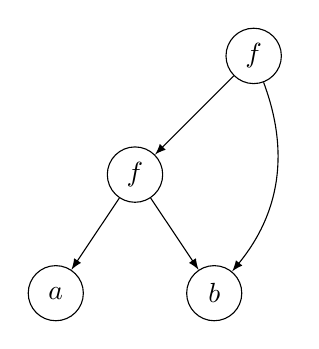
\begin{tikzpicture}
    \node [vertex] (v1) {$f$};
    \node [vertex,below left=of v1] (v2) {$f$};
    \node [vertex,below left=of v2,xshift=0.50cm] (v3) {$a$};
    \node [vertex,below right=of v2,xshift=-0.50cm] (v4) {$b$};

    \path [edge] (v1) -- (v2);
    \path [edge] (v1) edge [bend left] (v4);
    \path [edge] (v2) -- (v3);
    \path [edge] (v2) -- (v4);
  \end{tikzpicture}
}

\begin{frame}
  \frametitle{Example of a Term Graph}

  \begin{columns}
    \begin{column}{0.5\textwidth}
      Term graph of the terms $f(f(a,b),b)$, $f(a,b)$, $a$ and $b$.
    \end{column}
    \begin{column}{0.5\textwidth}
      \exampleone{}
    \end{column}
  \end{columns}
\end{frame}

\begin{frame}
  \frametitle{Congruence}

  \begin{Definition}[Congruence]
    \begin{itemize}
      \item Let $R \subseteq V \times V$ be a relation.
      \item Two vertices $u$ and $v$ are \textit{congruent under $R$} iff
        \begin{itemize}
          \item $\lambda(u) = \lambda(v)$,
          \item $\sigma(u) = \sigma(v)$ and
          \item forall $i$ s.t. $1 \leq i \leq \sigma(u)$, $R(u[i],v[i])$.
        \end{itemize}
      \only<4->{
      \item $R$ is \textit{closed under congruences} if, forall vertices $u$ and
        $v$ s.t. $u$ and $v$ are \textit{congruent under $R$}, $R(u,v)$.
      }
    \end{itemize}
  \end{Definition}

  \pause

  \pgfdeclarelayer{background}
  \pgfdeclarelayer{foreground}
  \pgfsetlayers{background,main,foreground}
  \usebeamercolor{frametitle}

  \begin{tikzpicture}
    \node [vertex] (v1) {$x$};
    \node [vertex,right=of v1] (v2) {$x$};

    \node [vertex,left=of v4,xshift=+0.5cm] (v3) {$y_1$};
    \node [vertex,below=of v1,xshift=-0.4cm] (v4) {$z_1$};
    \node [vertex,below=of v2,xshift=+0.4cm] (v5) {$y_n$};
    \node [vertex,right=of v5,xshift=-0.5cm] (v6) {$z_n$};

    \path [edge] (v1) -- (v3);
    \path [edge] (v2) -- (v4);
    \path [edge] (v1) -- (v5);
    \path [edge] (v2) -- (v6);
    \path (v4) edge [draw=none] node {$\ldots$} (v5);

    \path [equality,beameralert=3] (v3) edge node [above] {$R$} (v4);
    \path [equality,beameralert=3] (v5) edge node [above] {$R$} (v6);

    \path [equality,beameralert=5] (v1) edge node [above] {$R$} (v2);

  \end{tikzpicture}
\end{frame}


\begin{frame}
  \frametitle{The Congruence Closure of $R$}

  \begin{Lemma}[Congruence Closure]
    There is a unique minimal extension $R'$ of $R$ s.t. $R'$ is an equivalence
    relation and $R'$ is closed under congruences; $R'$ is the
    \textit{congruence closure} of $R$.
  \end{Lemma}
\end{frame}

\section{Implementation}

\begin{frame}[fragile]
  \frametitle{$\mathbf{congruent}(u, v)$}

  \begin{columns}[T]
    \begin{column}{0.5\textwidth}
      \haskellfile
        [ firstline=115
        , lastline=120
        ]
        {../src/Logic/CongruenceClosure.hs}
    \end{column}
    \begin{column}{0.5\textwidth}
      \begin{enumerate}
        \item if $\sigma(u) \neq \sigma(v)$, then return $\mathbf{false}$
        \item for $1 \leq i \leq \sigma(u)$, if $\mathbf{find}(u[i]) \neq \mathbf{find}(v[i])$,
          then return $\mathbf{false}$
        \item return $\mathbf{true}$
      \end{enumerate}
    \end{column}
  \end{columns}
\end{frame}

\begin{frame}[fragile]
  \frametitle{$\mathbf{merge}(u,v)$}
  \framesubtitle{Produces the Congruence Closure of $R \cup \{(u,v)\}$}

  \begin{columns}[T]
    \begin{column}{0.5\textwidth}
      \haskellfile
        [ firstline=89
        , lastline=102
        ]
        {../src/Logic/CongruenceClosure.hs}
    \end{column}
    \begin{column}{0.5\textwidth}
      \begin{enumerate}
        \footnotesize
        \only<1>{
          \item If $\mathbf{find}(u) = \mathbf{find}(v)$, then return.
          \item Let $P_u$ be the set of all predecessors of all vertices equivalent
            to $u$, and $P_v$ the set of all predecessors of all vertices
            equivalent to $v$.
          \item Call $\mathbf{union}(u, v)$.
        }
        \setcounter{enumi}{3}
        \only<2>{
          \item For each pair $(x, y)$ such that $x \in P_v$, and $y \in P_o$, If
            $\mathbf{find}(x) \neq \mathbf{find}(y)$ but $\mathbf{congruent}(x, y) =
            \mathbf{true}$,
            then $\mathbf{merge}(x, y)$.
        }
      \end{enumerate}
      \begin{itemize}
        \only<3>{
          \item Runtime complexity of $\mathbf{merge}(x,y)$ is $O(n^2)$ where
            $n$ is the number of edges of the Graph.
          \item With a more sophisticated version of step 4, the runtime
            complexity can be reduced to $O(n \log n)$.
        }
      \end{itemize}
    \end{column}
  \end{columns}
\end{frame}

\begin{frame}[fragile]
  \frametitle{Example $\mathbf{merge}(f(a,b),a)$ }

  \begin{columns}[T]
    \begin{column}{0.4\textwidth}
      \only<2-> { \haskellfile [firstline=1,lastline=4] {figure1.trace} }
      \only<3-> { \haskellfile [firstline=5,lastline=8] {figure1.trace} }
    \end{column}
    \begin{column}{0.6\textwidth}
      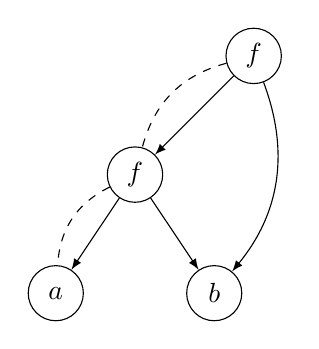
\begin{tikzpicture}
        \node [vertex] (v1) {$f$};
        \node [vertex,below left=of v1] (v2) {$f$};
        \node [vertex,below left=of v2,xshift=0.50cm] (v3) {$a$};
        \node [vertex,below right=of v2,xshift=-0.50cm] (v4) {$b$};

        \path [edge] (v1) -- (v2);
        \path [edge] (v1) edge [bend left] (v4);
        \path [edge] (v2) -- (v3);
        \path [edge] (v2) -- (v4);

        \path [equal,beameralert=2] (v2) edge [bend right] (v3);
        \path [equal,beameralert=3] (v1) edge [bend right] (v2);
      \end{tikzpicture}
    \end{column}
  \end{columns}
\end{frame}

\begin{frame}[fragile]
  \frametitle{$\mathbf{decisionProcedure}(\Phi)$ and correctness}
  %\framesubtitle{}

  \haskellfile
    [ firstline=77
    , lastline=85
    ]
    {../src/Logic/CongruenceClosure.hs}

  \pause

  \haskellfile
    [ firstline=123
    , lastline=128
    ]
    {../src/Logic/CongruenceClosure.hs}
\end{frame}

\begin{frame}[fragile]
  \frametitle{Example $f(a,b) = a \rightarrow f(f(a,b),b) = a$ }

  \setlength{\parindent}{0pt}
  \haskellfile
    [ firstline=38
    , lastline=42
    ]
    {../src/Logic/CongruenceClosure.hs}

  \begin{columns}[T]
    \begin{column}{0.4\textwidth}
      \only<2-> { \haskellfile [firstline=1,lastline=4] {figure1.trace} }
      \only<3> { \haskellfile [firstline=5,lastline=8] {figure1.trace} }
      \only<4> { \haskellfile [firstline=5,lastline=10] {figure1.trace} }
    \end{column}
    \begin{column}{0.6\textwidth}
      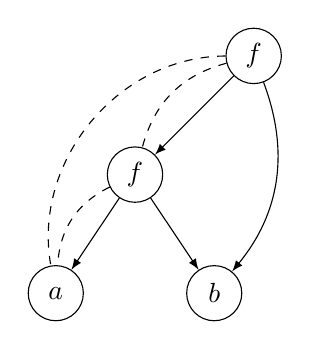
\begin{tikzpicture}
        \node [vertex] (v1) {$f$};
        \node [vertex,below left=of v1] (v2) {$f$};
        \node [vertex,below left=of v2,xshift=0.50cm] (v3) {$a$};
        \node [vertex,below right=of v2,xshift=-0.50cm] (v4) {$b$};

        \path [edge] (v1) -- (v2);
        \path [edge] (v1) edge [bend left] (v4);
        \path [edge] (v2) -- (v3);
        \path [edge] (v2) -- (v4);

        \path [equal,beameralert=2] (v2) edge [bend right] (v3);
        \path [equal,beameralert=3] (v1) edge [bend right] (v2);
        \path [equal,beameralert=4] (v1) edge [bend right=50] (v3);
      \end{tikzpicture}
    \end{column}
  \end{columns}
\end{frame}

\begin{frame}[fragile]
  \frametitle{Example $f^3(a) = a \land f^5(a) = a \rightarrow f^1(a) = a$ }

  \setlength{\parindent}{0pt}
  
  \begin{columns}[T]
    \begin{column}{0.4\textwidth}
      \haskellfile
        [ firstline=54
        , lastline=59
        ]
        {../src/Logic/CongruenceClosure.hs}
    \end{column}
    \begin{column}{0.6\textwidth}
      \scalebox{0.7}{
      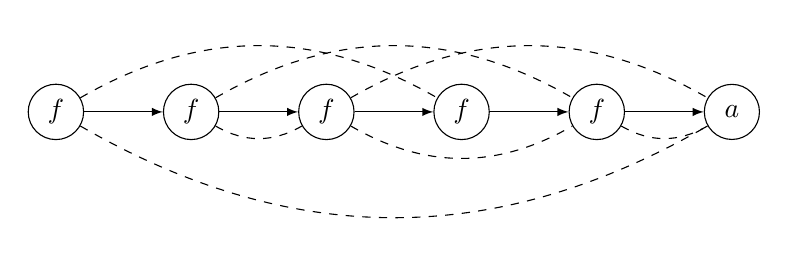
\begin{tikzpicture}
        \node [vertex] (v1) {$f$};
        \node [vertex,right=of v1] (v2) {$f$};
        \node [vertex,right=of v2] (v3) {$f$};
        \node [vertex,right=of v3] (v4) {$f$};
        \node [vertex,right=of v4] (v5) {$f$};
        \node [vertex,right=of v5] (v6) {$a$};

        \path [edge] (v1) -- (v2);
        \path [edge] (v2) -- (v3);
        \path [edge] (v3) -- (v4);
        \path [edge] (v4) -- (v5);
        \path [edge] (v5) -- (v6);

        \path [equal,beameralert=2] (v3) edge [bend left] (v6);
        \path [equal,beameralert=3] (v2) edge [bend left] (v5);
        \path [equal,beameralert=4] (v1) edge [bend left] (v4);
        \path [equal,beameralert=5] (v1) edge [bend right] (v6);
        \path [equal,beameralert=6] (v2) edge [bend right] (v3);
        \path [equal,beameralert=7] (v3) edge [bend right] (v5);
        \path [equal,beameralert=8] (v5) edge [bend right] (v6);
      \end{tikzpicture}
      }
    \end{column}
  \end{columns}

  \vspace{1cm}

  \only<2>{ \haskellfile [firstline=1,lastline=4] {figure2.trace} }
  \only<3>{ \haskellfile [firstline=5,lastline=8] {figure2.trace} }
  \only<4>{ \haskellfile [firstline=9,lastline=12] {figure2.trace} }
  \only<5>{ \haskellfile [firstline=13,lastline=16] {figure2.trace} }
  \only<6>{ \haskellfile [firstline=17,lastline=20] {figure2.trace} }
  \only<7>{ \haskellfile [firstline=21,lastline=21] {figure2.trace} }
  \only<8>{ \haskellfile [firstline=21,lastline=23] {figure2.trace} }
\end{frame}

\begin{frame}[fragile]
  \frametitle{Example $a \neq b \land b \neq c \land c \neq a \land a = d \land d = e$ }

  \haskellfile[] {figure3.trace}

  \pause

  $T/_\sim = \{ \{ a,d,e \}, \{ b \}, \{ c \} \}$
\end{frame}

\section{Extension for LISP}

\begin{frame}[t]
  \frametitle{Axioms of the QF theory of list structures}

  A small modification to the decision procedure allows to proof terms in the
  quantifier-free theory of LISP list structures.

  \begin{block}{Axioms}
    \vspace{-0.7cm}
    \begin{align*}
      \car{\cons{x,y}} &= x \\
      \cdr{\cons{x,y}} &= y \\
      \neg \atom{x} \subset \cons{\car{x}, \cdr{x}} &= x \\
      \neg \atom{\cons{x,y}} &
    \end{align*} \quad
  \end{block}
\end{frame}

\begin{frame}
  \frametitle{Adjustments to the decision procedure}

  \begin{itemize}
    \only<1>{
      \item For each term $\cons{x,y}$ in the term graph, $x = \car{\cons{x,y}}$
        and $y = \cdr{\cons{x,y}}$ is added as a conjunct to the input formula.
      \item Replace negative $\atom{t}$ by $t = \cons{u,v}$ where $u$ and $v$ are
        free in the input formula.
    }

    \item For an input formula of the form
      \begin{align*}
        & \atom{u_1} \land \ldots \atom{u_q}\ \land \\
        & v_1 = w_1 \land \ldots v_r = w_r\ \land \\
        & x_1 \neq y_1 \land \ldots x_s \neq y_s
      \end{align*}
      merge all $v_i$ and $w_i$ where $1 \leq i \leq r$.

    \only<2>{
      \item Unsatisfiable if
        \begin{itemize}
          \item any $x_j$ equivalent to $y_j$ where $1 \leq j \leq s$
          \item the equivalence class of any $u_k$ contains a vertex labeled $\cons{\ldots}$ where $1 \leq k \leq q$
        \end{itemize}
      \item Otherwise satisfiable
    }
  \end{itemize}
\end{frame}

\begin{frame}
  \frametitle{NP-completeness of a different theory}

  If the axioms of the theory are slightly modified, the decision procedure
  becomes NP-complete

  \pause

  \begin{block}{Axioms}
    \vspace{-0.7cm}
    \begin{align*}
      \car{\cons{x,y}} &= x \\
      \cdr{\cons{x,y}} &= y \\
      x \neq \nil{} \supset \cons{\car{x}, \cons{x}} &= x \\
      \cons{x,y} &\neq \nil{} \\
      \car{\nil{}} = \cdr{\nil{}} &= \nil{}
    \end{align*}
  \end{block}

  \pause

  Proof idea: Reduce the 3-CNF satisfiability problem for propositional calculus to
  the satisfiability problem of the modified LISP theory.
\end{frame}

\begin{frame}
  \frametitle{Proof: NP-completeness of a different theory}

  \begin{itemize}
    \only<1>{
      \item Let $F$ be a conjunction of three-element clauses over propositional
        variables $p_1, \ldots, p_n$.
    }

    \item Let $G$ a conjunction of equalities and disequalities of list
      structure terms over $2n$ variables $x_1,y_1,\ldots,x_n,y_n$:
      \begin{align*}
        \car{x_1} = \car{y_1} \land \cdr{x_1} &= \cdr{y_1} \land x_1 \neq y_1\ \land \\
        \vdots & \\
        \car{x_n} = \car{y_n} \land \cdr{x_n} &= \cdr{y_n} \land x_n \neq y_n \land \ldots
      \end{align*}
      Note: Either $x_i$ or $y_i$ must be $\nil{}$ and the other
      $\cons{\nil{},\nil{}}$.

    \only<1>{
      \item Given interpretation $\psi$ for $G$, construct interpretation $\phi$ for
        $F$, s.t. $\psi$ satisfies $G$ iff $\phi$ satisfies $F$. Define
        $\phi(p_i)$ is true iff $\psi(x_i) = \nil{}$.
    }

    \only<2>{
      \item The remaining part of $G$ contains conjuncts that guarantee the
        equisatisfiability of $F$ and $G$.
      \item Example: If $F$ contains a conjunct $p_1 \lor \neg p_2 \lor p_3$,
        add $x_1 = \nil{} \lor x_2 \neq \nil{} \lor x_3 = \nil{}$ to $G$
    }
  \end{itemize}
\end{frame}

\section{Conclusion}

\begin{frame}
  \frametitle{Conclusion}

  \begin{itemize}
    \item
      Congruence closure provides a fast decision procedure for the
      quantifier-free theory of equality over uninterpreted function symbols.

    \pause
    \item
      The decision procedure can be extended carefully to proof terms of
      advanced theories like the theory of list-structures.

    \pause
    \item
      Careless extensions can cause the decision procedure to become
      NP-complete.
  \end{itemize}
\end{frame}

\end{document}
